\section{Background}
\label{sec:background}

\subsection{Bitcoin}
\label{ssection:bitcoin}

The bitcoin protocol \cite{bitcoin-core} specifies a set of rules that enable the emergence of a decentralized, peer-to-peer payment network. This network is permissionless, meaning any node is able to join the network.\\
Every time a user wants to spend bitcoin he needs to create and then broadcast a transaction to the network. A bitcoin transaction consists of at least one input and one output, summarized formats for these data structures are depicted by Tables \ref{table:tx_input} and \ref{table:tx_output} \cite{bitcoin_protocol_doc}.

\begin{table}[H]
\centering
\resizebox{\columnwidth}{!}{\begin{tabular}{|l|l|}
\hline
\rowcolor[HTML]{C0C0C0} 
Field Name & Description \\ \hline
Transaction Hash & Hash of the transaction that includes the output to be spent \\ \hline
Output Index & The index number for the output to be spent \\ \hline
Unlock script & A script that unlocks the bitcoin
\end{tabular}}
\caption{Transaction input structure}
\label{table:tx_input}
\end{table}

\begin{table}[H]
\centering
\begin{tabular}{|l|l|}
\hline
\rowcolor[HTML]{C0C0C0} 
Field Name & Description \\ \hline
Value & Amount of bitcoin to be transferred \\ \hline
Locking script & A script that locks the bitcoin \\ \hline
\end{tabular}
\caption{Transaction output structure}
\label{table:tx_output}
\end{table}

When creating a transaction the user starts by picking one or more outputs to be spent, these are chosen by referring to a list of unspent outputs (UTXO) normally kept by each node. He then proceeds to create his own transaction inputs, one for each picked output. The inputs point to the output they are spending using the "Transaction Hash" and "Output Index" fields, proving the output can be spent by setting the "Unlocking script" field into a script that returns true when concatenated with the locking script of the output to be spent.
After proving that he can spend from the chosen outputs by creating the necessary inputs, the user should now dictate the new way in which the bitcoin should be spent, this is done by creating the new outputs that will be added to the UTXO. The amount of bitcoin that is locked by the outputs introduced by a new transaction should be smaller than the amount that was locked by the outputs referenced by the transaction inputs and the difference between these two values will correspond to the transaction fee.\\

\subsubsection{The Bitcoin Script language}
\label{sssec:bitcoin_script}

Script \cite{bitcoin_script} is a simple scripting language used to validate transactions in the bitcoin blockchain. It is used to dictate how the bitcoins sent to a certain user can be spent and helps validate the spending of such bitcoins by that user.\\
In Script there are two essential elements, data and operation codes (or opcodes) that serve as functions that handle the data, these are processed from the left to the right, making use of a stack. Data is always added to the stack while opcodes can result in data being added to or removed from the stack. A script is considered valid if there are no failures triggered during its execution and if when it exits the top item of the stack is not zero. \\
Figure \ref{fig:op_return} represents a simple OP\_RETURN script. This is a special type of script pattern, its goal is not to send any bitcoin but to store information in the blockchain.

\begin{figure}[H]
\begin{center}
  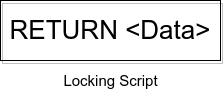
\includegraphics[width=0.3\linewidth]{images/op_return.png}
  \caption{RETURN script pattern}
  \label{fig:op_return}
  \end{center}
\end{figure}

The information stored by $<Data>$ is as tampering-proof as a bitcoin transaction and it will be readily available for any fully synced bitcoin node. The output associated with an OP\_RETURN locking script will never be able to be spent because the script's execution will fail as soon as the opcode RETURN is executed.

\subsubsection{Scalability Issues}

As it is currently designed, the bitcoin protocol is not capable of being adopted as a large scale VISA-like payment network. There is a limit, imposed by the consensus rules, on the maximum size of blocks. This imposes a maximum rate of growth for the blockchain and a ceiling on the number of transactions per second it can process. Estimates have pointed to bitcoin being able to handle 27 \cite{bitcoin_tps} transactions per second, much behind the 65,000 \cite{visa_tps} claimed by VISA. \\
Throughout bitcoin's existence work has been put into finding the best way for it to scale into a global payment network. Some proposals \cite{bch, bsv} have suggested raising the limit on the maximum size of blocks and consequently let more transactions fit in each block, effectively raising the maximum number of transactions per second but also raising the amount of bandwidth and computational capabilities needed to join the network and independently verify every transaction. Other types of proposals use a layered architectural approach, using bitcoin as the base layer and building on top of it.

\subsection{Lightning Network}
\label{ssec:lightning_network}

The Lightning protocol \cite{lightning_network} is a second layer protocol that is built on top of the bitcoin protocol. Using bitcoin's transaction scripting capabilities, Lightning defines the rules for the creation of a secondary overlay network between bitcoin nodes that allows for payments to be made from one node to another without trusting the intermediary nodes and without broadcasting new transactions to the blockchain. \\
The lighting network has two main elements, nodes and payment channels. Payment channels are created when two nodes decide to broadcast a \textit{Funding Transaction} and add it to the blockchain, each effectively committing a pre-determined amount of bitcoin to the payment channel they just created. They can then use the payment channel to transact between themselves privately at will, closing it and redeeming their bitcoin through another blockchain transaction whenever they wish to. \\
When the payment channel concept is extended to allow for payments between nodes that are not directly connected there is a need to create payment routes; paths composed of multiple payment channels where payments between the end nodes can be routed through without the need of broadcasting them to the entire network.

\subsection{Lightning Network Routing}
\label{ssec:lightning_network_routing}

Although the way in which the payment route is chosen is not defined by the lightning specifications \cite{lightning_network_specs} the original lightning whitepaper \cite{lightning_network} lays out some ideas on how routing could work. It suggests that the network will eventually look like the banking network it serves, with banks being the highly connected nodes. They would work similarly to the internet's Tier-1 \acrshort{isp}'s, maintaining high availability and using routing tables to help make connections between the more unreliable edge nodes such as average users. The topology of the network is turning out to be what the whitepaper suggested it would, exhibiting the properties of a scale-free network \cite{ln_analysis} \cite{network_science}. \\
It's interesting to understand that, much like in the internet, bitcoin is following a layered design principle, the bitcoin protocol stack can be thought of as currently composed of the bitcoin protocol serving as a base layer with the lightning network on top of it. As suggested by Figure \ref{fig:bitcoin_protocol_stack}, a \acrfull{lrp} would work on top of lighting as a third layer of the bitcoin stack.

\begin{figure}[H]
\begin{center}
  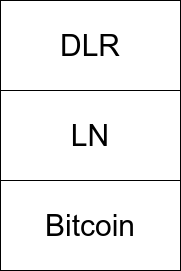
\includegraphics[width=0.5\linewidth]{images/protocol_stack.png}
  \caption{Bitcoin protocol stack}
  \label{fig:bitcoin_protocol_stack}
  \end{center}
\end{figure}

Every current implementation uses source routing, meaning that the route for a payment is entirely calculated by the sender. Source routing is advantageous in the sense that it preserves the anonymity of the sender and the receiver, preventing any routing node to censor the payment based on its origin or destination.\\
When calculating a payment path, the sender leverages the information he has about the topology of the network, gathered from watching the payment channels opening and closing through the transactions committed to the blockchain to run a version of the Dijkstra algorithm and construct a possible payment path. \\
After a route is successfully discovered the overlying payment can still be invalid or fail to be completed. The found route might span more than 20 hops (which collides with the current onion routing implementation), the channel might not have enough capacity for the payment, nodes in the payment route can be uncooperative or it might be the case that at least one of the channels in the route doesn't have the right distribution of funds. For example, given the distribution of funds in the payment channel shared by Alive and Bob and represented by Figure \ref{fig:payment_channel} it would be impossible for Charlie to build a valid payment route that allowed for a 2 BTC payment and included the channel in the direction Alice-Bob, this is because Alice has a channel balance of 1 BTC and wouldn't be able to route the payment through. It would, however, and since Bob can send a maximum of 3 BTC to Alice, be possible to find a route for that payment that uses the payment channel in the Bob-Alice direction. 

\begin{figure}[H]
\begin{center}
  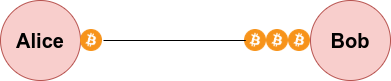
\includegraphics[width=0.6\linewidth]{images/alice_bob_channel.png}
  \caption{Alice's and Bob's payment channel. It has a capacity of 4 BTC and the state
(Alice: 1 BTC, Bob: 3 BTC)}
  \label{fig:payment_channel}
  \end{center}
\end{figure}

Although some details about the channels and a local view of the network's topology are maintained through the peer-to-peer exchange of the gossip messages defined by the specification, a node does not possess any information about the distribution of funds in channels in which it does not take part. The fact that the information on these channel states is held privately by the partakers of each channel preserves a degree of privacy in the network while diminishing the efficiency of the routing process. \\
A previous analysis of the lightning network \cite{ln_analysis} concluded that when using the current Dijkstra shortest path algorithm for route finding a small increase in the volume of a payment sharply decreases its probability of success. This happens because as a payment gets larger it's harder for it to "fit" in a valid payment route, it gets more and more likely that one of the channels that make up the path doesn't have the right balance distribution to allow the payment to go through. Using this routing algorithm ends up wasting much of the network channels' capacity which could be put to better use if accounted for when defining the payment's route.

\subsubsection{Flare}
\label{sssec:flare}

Flare \cite{flare} explores the ideas behind routing in \acrfull{manet} and applies them to routing in the lighting network.\\
\acrshort{manet}s share a lot of similarities with the lighting network. Like what happens with payment channels the connections between nodes in \acrshort{manet}s are unstable, being created and becoming unavailable frequently. The same happens with nodes that, much like lighting nodes, recurrently join and leave the network. This frequent changes in the network make its topology very dynamic and an interesting study case for how routing in lighting might work. \\
Flare is characterized as a hybrid routing algorithm. It is composed of two complementary proactive and reactive parts.\\
The proactive part is responsible for keeping an updated routing table with information about channels in the local neighbourhood of the node but also information about beacon nodes. Any node can be a beacon node and every node has a different set of different nodes, they are assigned randomly and are scattered across the network, they help a node find paths beyond its neighbourhood by increasing the node's visibility of the network. A proactive scheme like this guarantees a strong knowledge of the local neighbourhood with the possibility of making connections with nodes further away. \\ 
The reactive part of the algorithm takes the stage when a node decides to make a payment over \acrshort{ln}. If Alice wants to pay Bob she first tries to find a path that doesn't require a beacon node, this is accomplished by combining Bob's and her own routing table to find common known nodes. \\
If it is not possible to find a path to Bob by combining their routing tables Alice will contact a beacon node and request his routing table to try to find a path to Bob in it. Due to how the proactive part of the algorithm works it is more probable to find a path by contacting these beacon nodes than by contacting any other nodes in the network. If Alice can't find a path by contacting the first beacon node she will sequentially try the other beacon nodes available in her routing table.\\
Flare nodes rely on special "beacon" nodes to find paths to other nodes outside their neighbourhood. This is a threat to decentralization (the capacity of having all nodes performing the same tasks and having access to the same information) because it means that some nodes will have more information and perform different tasks than the rest of the network. Besides, and according to simulation, the dependence on beacons gets even larger as more beacons join the network. \\
Simulations using Flare in a 100,000 nodes network found that it was able to find paths from 10 random nodes to every node in the network using the minimum of 5 beacons while keeping less than an average of 1000 routing entries per routing table \cite{flare}. The discovered paths are mostly suboptimal since the process of discovering new beacons to be able to communicate with nodes further away is depth-first search based. All the simulations considered a Watts-Strogatz graph \cite{watts-strogatz} which dismisses the scale-free properties presented by the network which might not have been apparent at the time of publication.\\

\subsubsection{Ant Routing}

The Ant routing algorithm for the Lightning Network \cite{ant_routing} is a decentralized payment pathfinding algorithm inspired by ant path searching algorithms. These are based on the fact that when ants distribute themselves through paths to a destination, they tend to accumulate more pheromones in the faster paths, leading to a positive loop that leads to most ants choosing the longer path.\\
As opposed to Flare (\ref{sssec:flare}) Ant Routing doesn't rely on any nodes having a privileged view over the network, instead, it works under the assumption that every node will have the access to the same information, increasing decentralization. \\
When Alice wants to pay Bob they agree on a random large number called the \textit{derived seed} and denoted by $S'$. Then they each concatenate their own bit with the derived seed to get their own \textit{pheromone seed}, represented by $S$. Alice's pheromone seed would be the concatenation of the bit "0" with the derived seed and Bob's would result from the concatenation of bit "1" with the derived seed. 
For every pheromone seed $S$ there's a \textit{conjugate seed}, denoted by $\overline{S}$ and defined as the pheromone seed with the same derived seed but a different initial bit.\\
After Alice and Bob have created their pheromone seeds they send them to the peers with whom they share a payment channel. \\
Every node keeps a database with all the pheromone seeds they have received until moment $T$. If at moment $T+1$ a node receives a new seed it checks if it's the matching conjugate seed of a pheromone seed it has in memory; if it isn't the new seed is added to the database and broadcast to the node's neighbours, if it is, it means that a path between two nodes has been found. When this happens the node that did the matching will build a matched seed that will be relayed through the network until it reaches the node that sent the corresponding pheromone seed. The node that receives the matched seed, let's say it was Alice, then builds a confirmed seed from the matched seed and sends it, through each one of the path's hops, to Bob, who confirms with Alice having received it, allowing her to start the payment in the lighting network using the path they just found. \\
This routing algorithm successfully keeps the decentralization of the network by having all nodes performing the same tasks. It preserves a high level of anonymity since no node outside payment path knows about the payment and the nodes in the payment path who route the payment don't know anything about its origin or destination. \\
Having to frequently broadcast pheromone seeds through the network increases the computational and bandwidth needs of the network which might be problematic in a situation where there's a very dense network graph and the fact that the scale-free topology of the network is not considered by the algorithm is also undesirable since it leaves out important information which could improve its performance. \\
Ant Routing was estimated to be able to sustain a number of transactions per second in the order of the several thousand \cite{ant_routing_scalability} which could cover most of the world's payment processing needs.

\subsection{Distance-vector Routing}
\label{ssec:distancevectorrouting}

A distance vector routing protocol is characterized by the existence of a routing table in each node \cite{distance_vector}. This table contains the distance between the node and every other destination on the network as well as the next hop needed in order to reach the destination at that distance. \\
Table \ref{table:dv_routing_table_a} represents node A's routing table from the network in Figure \ref{fig:dv_networkabcd}, after the algorithm converges.

\begin{figure}[H]
\begin{center}
  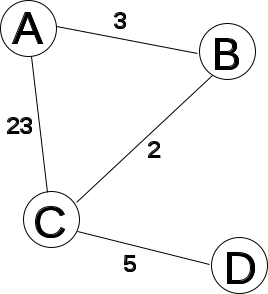
\includegraphics[width=0.4\linewidth]{images/networkabcd.png}
  \caption{Example Routing Network. Reprinted from \cite{distance_vector}.}
  \label{fig:dv_networkabcd}
  \end{center}
\end{figure}

\begin{table}[H]
\centering
\begin{tabular}{|l|l|l|}
\hline
\rowcolor[HTML]{C0C0C0} 
Destination & Distance & Next Hop \\ \hline
B           & 3    & B        \\ \hline
C           & 5    & B        \\ \hline
D           & 10   & B        \\ \hline
\end{tabular}
\caption{Node A's Routing Table}
\label{table:dv_routing_table_a}
\end{table}

Nodes periodically share their routing table with their neighbours. Updates to the routing table sent by a neighbouring node might contain new information about the networks dynamic topology or information about an updated distance value. When a new table is received it's combined with the local table which is updated if new destinations or shorter paths to known destinations are found. \\
As opposed to every other routing algorithm presented in section \ref{ssec:lightning_network_routing}, distance-vector routing is not a source routing scheme. Routes are not entirely decided by the source node, instead, this job is divided by the nodes the route who decide, based on their "Next Hop" table entries, what the next hop in the path to a certain destination will be, with every node in the path doing this until the destination is reached. \\
